Uma das principais dificuldades encontradas no problema da mochila multiobjetivo
é a grande cardinalidade do \paretoset{}.
De fato, grande parte dos problemas multiobjetivos são considerados \emph{intratáveis},
no sentido de possuir uma quantidade exponencial de soluções eficientes
dado o tamanho da instância~\cite{ehrgott2013multicriteria}.
Esta causa tem motivado pesquisadores
a desenvolverem métodos heurísticos, que computam aproximações deste conjunto
demandando menor esforço computacional quando comparado aos métodos exatos.
%~\cite{bazgan2015approximate, vanderpooten2017covers}.

A maioria das heurísticas propostas para problemas multiobjetivo
são adaptações de meta-heurísticas originalmente propostas para
problemas de otimização escalar.
Dentre esses métodos vale mencionar o algoritmo de recozimento simulado
~\cite{czyzzak1998pareto},
o algoritmo de busca dispersa~\cite{da2006scatter,da2007integrating},
algoritmo de busca tabu~\cite{gandibleux2000tabu},
algoritmo imunológico artificial~\cite{gao2014quantum},
algoritmo genético~\cite{abdelaziz1999hybrid}
e o algoritmo de estimação de distribuição~\cite{martins2017hybrid}.

Uma das heurísticas mais populares para o MOKP é o algoritmo genético
de ordenação não dominada (NSGA-II) proposto em~\cite{deb2002fast}.
O NSGA-II se diferencia das primeiras propostas de algoritmos evolucionários
multiobjetivo por utilizar uma estratégia mais eficiente
de ordenação de soluções dominantes e, consequentemente de
definição de aptidão do indivíduo.
O processo de ordenação de soluções dominantes agrupa as soluções
em conjuntos ordenados, chamados \emph{frontes não dominados},
nos quais as soluções dos primeiros conjuntos não são dominadas pelas soluções dos conjuntos seguintes.
A estratégia consiste em realizar um pré-processamento sobre o conjunto de
soluções, no qual são computados para cada solução $x$ dois parâmetros: a quantidade de soluções
que dominam $x$ e o conjunto de soluções dominadas por $x$.
Este pré-processamento permite a otimização do procedimento de ordenação.
Sendo $\np{}$ o número de objetivos e $N$ o tamanho da população,
o procedimento de ordenação proposto requer apenas $\mathcal{O}(\np{}N^2)$ comparações
enquanto que os procedimentos anteriormente utilizados demandavam $\mathcal{O}(\np{}N^3)$ comparações.

Com o objetivo de manter a diversidade das soluções,
o NSGA-II também propõe a utilização de uma métrica de distância entre os indivíduos da população
baseada na média das distâncias entre uma solução e suas
vizinhas imediatas pertencentes ao mesmo fronte não dominado.
A média calculada caracteriza uma espécie de \emph{medida de aglomeração}.
Soluções rodeadas por outras soluções próximas possuem um alto valor de aglomeração,
enquanto soluções que apresentam uma vizinhança distante possuem baixo valor de aglomeração.
O algoritmo então tende a dar preferência às soluções com menor valor de aglomeração,
uma vez que manter soluções com alto valor de aglomeração tende a diminuir a diversidade do conjunto de soluções.
O NSGA-II então implementa um algoritmo genético com abordagem elitista,
%Inicialmente uma população de $N$ indivíduos é criada.
%Em seguida uma nova população de $N$ indivíduos é gerada a partir da população anterior.
%Os indivíduos da nova população juntamente com os da população anterior têm suas aptidões computadas
%através da ordenação em frontes não dominados.
%Os $N$ indivíduos com melhor valor de aptidão são então selecionados,
considerando quando necessário, a métrica proposta como critério de desempate.

Outra heurística popular para o MOKP é o algoritmo evolucionário de pareto robusto
(SPEA-II), proposto em~\cite{zitzler2001spea2}.
O SPEA-II mantém durante o processo de otimização um conjunto de tamanho limitado,
desassociado da população corrente, contendo soluções não dominadas encontradas durante o processo.
Este conjunto, chamado de \emph{arquivo externo}
ou somente \emph{arquivo} (\emph{external archive} ou \emph{archive} em inglês)
é atualizado ao final de cada etapa de evolução, quando os melhores
indivíduos da população corrente são tomados como candidatos para inserção nesse arquivo.

O SPEA-II também propõe utilizar um valor refinado de aptidão.
Para as soluções não-dominadas, o valor de aptidão é associada
ao número de soluções da população que são dominadas pela respectiva solução.
Para os indivíduos dominados, o valor de aptidão é calculado com base nos valores de aptidão
das respectivas soluções dominantes.
Como critério de desempate é utilizada uma métrica de densidade, baseada na distância
até os $k$ vizinhos mais próximos.
Assim que o processo evolutivo se encerra, o SPEA-II retorna o arquivo externo como sendo a aproximação do \paretoset.

Outro algoritmo heurístico popular, para o qual se relata os melhores desempenhos para o MOKP,
é o algoritmo multiobjetivo evolucionário baseado em decomposição (MOEA/D)~\cite{zhang2007moea}.
O MOEA/D decompõe o problema original em $N$ subproblemas escalares, utilizando
um vetor de coeficientes de agregação.
Esses $N$ subproblemas são solucionados
através da evolução simultânea de $N$ populações, uma população para cada subproblema.
A cada geração a população é composta pelo melhor indivíduo encontrado até o momento
para aquele determinado subproblema, o que garante a convergência em direção ao \paretoset{}.
Além disso são definidas relações de vizinhança entre os subproblemas, baseadas
nas distâncias entre seus vetores de agregação.
Durante o processo de evolução, são utilizadas informações de subproblemas vizinhos,
fazendo com que dois subproblemas vizinhos tenham soluções similares.
O trabalho ainda discute diferentes estratégias para se definir os vetores de agregação.

Recentemente foi proposta uma heurística cooperativa para o MOKP baseado
em inteligência de enxame (MOFPA)~\cite{zouache2018cooperative},
apresentando resultados superiores às demais heurísticas.
O MOFPA combina a estratégia de movimento utilizada na otimização
por enxame de partículas com a estratégia de movimento
utilizada pelo algoritmo de otimização por colônia de vaga-lumes.
O algoritmo mantém uma população de indivíduos cujas posições
são atualizadas segundo a influência de outros indivíduos da população,
em uma movimentação par-a-par.
A estratégia de movimento a ser aplicada é definida
segundo a relação de dominância entre os dois indivíduos:
caso o indivíduo a ser movimentado domine o outro, o cálculo de movimento
é feito segundo o método de otimização por enxame de partículas,
caso contrário, o indivíduo é movimentado segundo o cálculo de atratividade
entre indivíduos, definido pelo algoritmo de colônia de vaga-lumes.
Visto que o movimento dos indivíduos ocorre em um espaço
contínuo, uma função de transição é aplicada para discretização da solução.
A estratégia de arquivo externo de soluções não dominadas
é utilizada para garantir as melhores soluções encontradas durante o processo de evolução,
assegurando assim a convergência do método em direção ao \paretoset{}.
Segundo os resultados computacionais apresentados,
o MOFPA foi capaz de gerar soluções
que superam diversas soluções estabelecidas pelos métodos anteriores.

\missingf{Eu acho que passa assim, mas vc está perdendo oportunidade de dar um maior volume na sua tese.
Como vc utiliza esses algoritmos nos experimentos poderia detalhar mais a sua descricao. Apresentar os algoritmos. Nao deve ser tao detalhado qto o do SCE mas pode ser bem mais detalhado do que vc fez. Sua tese está com 55 paginas... Tem que ser algo muito bom (com bons resultados) para passar sem problemas.

\resp Eu não utilizei nenhum dos algoritmos, utilizei apenas os resultados que o Zouache me enviou por email.

F: K, não utilizou, mas se explicar bem como funciona ajuda quem lê a compreender o que esses algoritmos fazem e o que o seu nao faz.

Sim, vou detalhar mais cada um deles. Cerca de três parágrafos para cada algoritmo, está bom?

F: Acho pouco mas melhor que nada. Prefiriria que incluisse os algoritmos na descricao.

}

Uma das propostas do presente trabalho é a implementação de um algoritmo evolutivo
populacional chamado algoritmo de evolução estocástica por complexos,
\emph{shuffled complex evolution} (SCE) em inglês,
para o problema da mochila multiobjetivo.
O SCE é uma heurística evolutiva robusta que surgiu como proposta
de solução para problemas hídricos de modelagem complexa~\cite{duan1992effective} e
deste então tem sido utilizada em outros problemas de otimização escalar.
Na seção seguinte o SCE será apresentado bem como as propostas de adaptação para ser aplicado ao
caso multiobjetivo e de implementação para o MOKP.

Esta proposta de implementação do algoritmo SCE para o MOKP será utilizada para testar o
desempenho da indexação multidimensional para o MOKP no contexto heurístico.
Visando validar a heurística proposta, sua performance com relação à qualidade de solução
também será comparada às principais heurísticas da literatura, cujos resultados serão
apresentados no Capítulo~\ref{cap:exp}.

\subsection{Evolução Estocástica por Complexos}

O Algoritmo de evolução estocástica por complexos (SCE)
é um algoritmo evolutivo populacional originalmente proposto por Duan~\cite{duan1992effective}
para auxiliar o planejamento de modelos de escoamento de águas pluviais.
Esse algoritmo tem sido utilizado com sucesso em diversos problemas como
seleção de projetos~\cite{elbeltagi2007modified},
problemas de escalonamento \cite{zhao2015shuffled},
problema da mochila $0-1$~\cite{bhattacharjee2014shuffled} e
problema da mochila multi-dimensional~\cite{baroni2015shuffled,baroni2016shuffled}.

O SCE é inspirado na evolução natural que ocorre de forma simultânea em
comunidades independentes.
A Figura~\ref{img:flow1} apresenta um fluxograma resumido do SCE.
O algoritmo trabalha com uma população particionada em $N$ comunidades,
ou complexos, cada uma contendo $M$ indivíduos.
Inicialmente a população de $N*M$ indivíduos é tomada aleatoriamente do espaço
de soluções viáveis.
Após essa inicialização, a população é ordenada em ordem decrescente de aptidão
e o melhor global é identificado.
Toda a população é então particionada em $N$ complexos, cada um contendo $M$ indivíduos.
Nesse processo de distribuição ocorre uma operação de \emph{embaralhamento} (\emph{shuffling} em inglês)
dos indivíduos, no qual o primeiro indivíduo é incluído no primeiro complexo,
o segundo indivíduo no segundo complexo, o $M$-ésimo
indivíduo no $M$-ésimo complexo, o $M+1$-ésimo indivíduo no primeiro complexo,
e assim por diante.

O próximo passo após a distribuição dos indivíduos em complexos é evoluir cada
complexo $K'$ vezes, sendo $K'$ uma constante.
Nesse processo, considerando que os indivíduos em cada complexo estão ordenados
em ordem decrescente de aptidão, um subcomplexo de $P$ indivíduos é selecionado
dentre o respectivo complexo, utilizando uma distribuição triangular, em que o $i$-ésimo
indivíduo tem a probabilidade $p_i = \frac{2(n+1-i)}{n(n+1)}$ de ser selecionado.
A utilização da distribuição triangular tem por objetivo priorizar os indivíduos
com melhor aptidão, favorecendo assim a convergência do algoritmo.

Após a seleção do subcomplexo, o seu pior indivíduo é identificado para ser
substituído por um novo indivíduo.
Esse novo indivíduo é gerado através do cruzamento do pior com um outro
de melhor aptidão.
Primeiramente o melhor indivíduo do subcomplexo é considerado.
Caso o indivíduo gerado não seja melhor que o pior selecionado,
o melhor indivíduo do complexo é então usado no cruzamento.
Se esse último cruzamento não resultou em melhoria, o melhor indivíduo de toda
a população é utilizado.
Finalmente, se todos os cruzamentos não foram capazes de gerar um melhor indivíduo,
esta pior solução selecionada é substituída por um novo indivíduo retirado de
forma aleatória do espaço de soluções viáveis.
Esse último procedimento é importante para impedir que o algoritmo fique
\emph{preso} num ótimo local.
O procedimento de evolução descrito acima é apresentado no fluxograma da Figura~\ref{img:flow2}.

\begin{figure}
  \centering
  \begin{minipage}[b]{0.42\textwidth}
    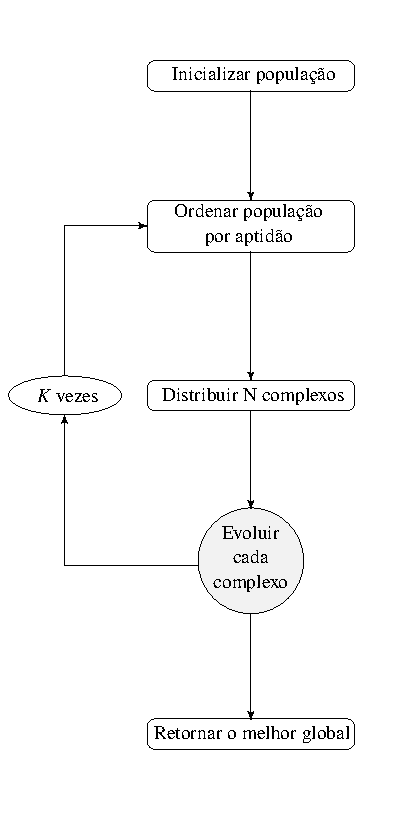
\includegraphics[width=\textwidth]{img/sce/flow1}
    \caption{Algoritmo de evolução estocástica por complexos.}
    \label{img:flow1}
  \end{minipage}
  \hfill
  \begin{minipage}[b]{0.42\textwidth}
    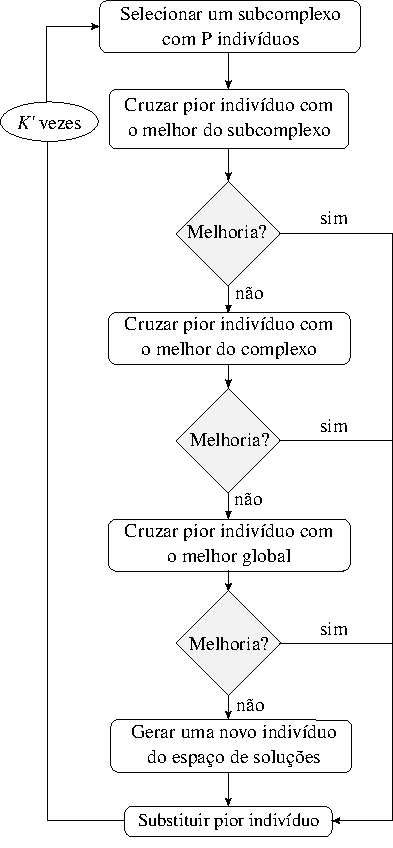
\includegraphics[width=\textwidth]{img/sce/flow2}
    \caption{Etapa de evolução executada para cada um dos complexos.}
    \label{img:flow2}
  \end{minipage}
\end{figure}

Após evoluir todos os $N$ complexos toda a população é novamente ordenada
em ordem decrescente de aptidão e o processo continua até que a condição
de parada seja satisfeita.
Destaca-se que no fluxograma da Figura~\ref{img:flow1} a condição de parada é a
execução de uma quantidade fixa de $K$ evoluções.

Uma das adaptações necessárias para se aplicar o SCE a um problema multiobjetivo
é a redefinição de métrica de qualidade de solução (aptidão),
uma vez que esta não é explícita como no caso da otimização escalar.
A métrica utilizada nesta proposta será a mesma adotada por heurísticas como NSGA-II e MOFPA,
a qual se baseia na ordenação não dominada (\emph{nondominated sorting}, em inglês)
das soluções, por apresentarem os melhores resultados relatados na literatura.

A ordenação não dominada agrupa as soluções em conjunto chamados \emph{frontes não dominados},
os quais possuem uma ordenação de dominância entre si. O primeiro fronte é formado
pelas soluções não dominadas.
Já o segundo fronte é formado pelas soluções dominadas apenas pelo primeiro fronte.
O terceiro fronte, por sua vez, é formado pelas soluções dominadas pelo primeiro
e segundo fronte, e assim sucessivamente.
Dessa forma as soluções dos frontes anteriores são consideradas superiores às soluções
dos frontes posteriores.

O Algoritmo~\ref{alg:frontsort} apresenta o algoritmo proposto por~\cite{deb2002fast}
e utilizado neste trabalho para ordenar as soluções em frontes não dominados.
A primeira fase do algoritmo é apresentada nas linhas 2 a 8,
onde algumas informações são pré-computadas.
Nas linhas 9 a 17 executa-se a segunda fase do algoritmo, onde as soluções são finalmente agrupadas
nos frontes.
Primeiramente são inicializados para cada solução $i$
os contadores de soluções dominadas $n_i$ (linha 2) e
o conjunto de soluções dominantes $B_i$ (linha 3).
Em seguida é feita uma comparação par-a-par através dos laços das linhas 4 e 5
para verificar se uma solução domina a outra (linha 6).
Caso isso aconteça, o contador de soluções dominantes e o conjunto de suas soluções dominadas
é atualizado.
Em seguida é definido o primeiro fronte de pareto, formado pelas soluções
não dominadas por nenhuma outra, ou seja, soluções que tem $n_i = 0$ (linha 9).
Enquanto houver alguma solução com ao menos uma solução dominante registrada (linha 11)
o algoritmo define um novo fronte (linhas 12 a 16).
Para cada solução que compõe o fronte anterior (linha 13), a lista de soluções dominadas
é visitada (linha 14), decrementando-se seus contadores de dominantes (linha 15).
Esse último passo faz com que a contagem de soluções dominantes $n_i$ desconsidere
as soluções recém agrupadas.
Na linha 16 o novo fronte é definido.
Quando todas as soluções estiverem agrupadas em frontes, o algoritmo é encerrado,
retornando a lista de frontes.

\begin{algorithm}
  \Kw{$A = (a_1, \ldots, a_q):$ conjunto de soluções }
\KwResult{$(F_1, \ldots, F_k ):$ Lista de frontes de pareto }
\Begin{
  $n_1, \ldots, n_q \gets 0$;\\
  $B_1, \ldots, B_q \gets \{\}$;\\
  \For{ $i \gets 1 : q$ }{
    \For{ $j \gets 1 : q$ }{
      \If{$a_i \;\dom\; a_j$}{
        $n_j \gets n_j + 1$;\ \mycomment[7.2mm]{ quantidade de soluções que dominam $a_j$ }
        $B_i \gets B_i \cup \{a_j\}$;\ \mycomment[1.2mm]{ conjunto das soluções dominadas por $a_i$ }
      }
    }
  }
  $ k \gets 1$;\\
  $F_1 \gets \{ a_i \in A \;|\; n_i = 0\}$;\ \mycomment[6.5mm]{ soluções não-dominadas (1º fronte) }
  \While{$\exists i \in \{1, \ldots, q\} \;|\; n_i > 0$}{
    $k \gets k + 1$\;
    \For{$a_i \in F_{k-1}$}{
      \For{$ a_j \in B_i$}{
        $n_j \gets n_j - 1$;\ \mycomment[7.2mm]{atualizando contagem}
      }
    }
    $F_k \gets \{ a_i \in A \;|\; n_i = 0\}$;\ \mycomment{formação do kº fronte}
  }
  \textbf{return} $(F_1, \ldots, F_k)$\;
}
  \caption{Algoritmo de ordenação de soluções em frontes não dominados.}
  \label{alg:frontsort}
\end{algorithm}

\begin{figure}
  \centering
  \begin{minipage}[t]{0.48\textwidth}
    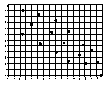
\includegraphics[width=\textwidth]{img/sce/unrankpop}
    \caption{População sem ordenação.}
    \label{img:unrankpop}
  \end{minipage}
  \hfill
  \begin{minipage}[t]{0.48\textwidth}
    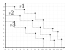
\includegraphics[width=\textwidth]{img/sce/rankpop}
    \caption{População ordenada em frontes não dominados.}
    \label{img:rankpop}
  \end{minipage}
\end{figure}

A Figura~\ref{img:unrankpop} apresenta um exemplo de população
para um problema bi-objetivo sem estarem ordenadas.
A Figura~\ref{img:rankpop} apresenta esta mesma população agora ordenada, ou seja, agrupada em frontes não dominados, conforme computado pelo Algoritmo~\ref{alg:frontsort}.

O desempate de aptidão entre indivíduos do mesmo fronte é feito pelo
valor de \emph{hiper-volume} de cada solução, como sugerido em~\cite{auger2012hypervolume}, por ser uma métrica
que exige pouco esforço computacional e tende a prover um \paretoset{} de melhor qualidade.
O hiper-volume de uma solução $x$ de um problema $\np$-objetivo
é dado por $\prod_{i=1}^{\np} f_i(x)$ e representa o volume multidimensional
dominado pela solução.
As soluções de um mesmo fronte mas, porém, com maior hiper-volume, serão consideradas
superiores as com menor hiper-volume. 

Uma última adaptação necessária para o SCE ser aplicado a problemas multiobjetivo
é em relação ao retorno do algoritmo, que deve ser um conjunto de soluções não dominadas,
representando uma aproximação do \paretoset{}, ao invés de apenas uma solução apenas.
Para que isso seja possível, será utilizada a estratégia de arquivo externo,
o qual será atualizado a cada final de etapa de evolução.
O Algoritmo~\ref{alg:archupdate} apresenta o procedimento de atualização do arquivo,
dada uma nova solução candidata.

\begin{algorithm}
  \Kw{$A:$ arquivo, $x:$ indivíduo }
\Begin{
  \If{$\nexists (y \in A, y \dom x)$}{
    $A \gets A \cup \{x\}$; \mycomment[1.7cm]{Inclusão de $x$ no arquivo}
    $A \gets A \backslash \{z \in A \;|\; x \dom z\}$; \mycomment{Remoção das soluções dominadas por $x$}
  }
  \textbf{return} $A$\;
}
  \caption{Procedimento de atualização de arquivo, dada uma nova solução.}
  \label{alg:archupdate}
\end{algorithm}

O Algoritmo~\ref{alg:archupdate} recebe como entrada o conjunto arquivo $A$ e uma solução
candidata $x$.
Primeiramente o algoritmo verifica se a solução $x$ é não dominada pelo arquivo, ou seja,
se não existe nenhuma solução $y \in A$ que domine $x$ (linha 2).
Em caso verdadeiro, dois passos são executados: $x$ é adicionado ao arquivo (linha 3) e
são retiradas do arquivo as soluções dominadas por $x$ (linha 4).
Finalmente o arquivo atualizado é retornado (linha 5).

%\section{O SCE para o MOKP}
Com a utilização do arquivo externo e a definição de aptidão baseada na ordenação
não dominada, o SCE está adaptado para resolver problemas multiobjetivo.
Entretanto, para se aplicar o SCE especificamente ao MOKP, ainda se faz necessário
definir dois procedimentos: o procedimento de criação de uma nova solução aleatória viável
e o procedimento de cruzamento entre duas soluções.
Os procedimentos utilizados neste trabalho para a construção de uma solução aleatória e
para o cruzamento de duas soluções são descritos nos Algoritmos~\ref{alg:new}
e \ref{alg:cross} respectivamente.

\begin{algorithm}
  \Begin{
  $v \leftarrow $ shuffle($1, 2, \ldots, n$)\;
  $s \leftarrow \vec{0}$; \Comment{solução vazia}\\
  \For{$ i \leftarrow 1:n$ }{
    $s[v_i] \leftarrow 1$; \Comment{inserção de item}\\
    \If{ $w(s) > W$ }{
      $s[v_i] \leftarrow 0$; \Comment{verificação de viabilidade}\\
    }
  }
  \textbf{retorna} $s$\;
}
  \caption{Construção de solução aleatória para o MOKP.}
  \label{alg:new}
\end{algorithm}

O Algoritmo~\ref{alg:new} primeiramente ordena
os índices dos $n$ itens numa ordem aleatória e
armazena-os em uma lista $v$ (linha 2).
Após a definição de uma nova solução vazia (linha 3), o algoritmo tenta de forma
iterativa preencher a solução com um item retirado da lista de índices (linhas 4-9).
A viabilidade da solução é então verificada: se o item inserido tornar a solução
inviável, ou seja, exceder a capacidade da mochila (linha 6), ele é então retirado
da solução (linha 7).
Após testar a inserção de todos os itens, a solução construída é retornada.

\begin{algorithm}
  \Kw{$x:$ pior indivíduo, $y:$ melhor indivíduo, $c$: número de genes herdados}
\Begin{
  $v \leftarrow $ shuffle($1, 2, \ldots, n$)\;
  $z \leftarrow \ord^{max}_{rev}$\;
  \For{$i \leftarrow 1:c$ }{
	  $x[v_i] \leftarrow y[v_i];$\ \Comment{herança de genes}
  }
  \For{$i \gets 1:n$ \textbf{and} $w(x) > W$}{
    $x[z_i] \gets 0;$\ \Comment{reparo de solução}
  }
	Computar aptidão de $x$\;
  \textbf{return} $x$\;
}
  \caption{Procedimento de cruzamento entre duas soluções do MOKP.}
  \label{alg:cross}
\end{algorithm}

O procedimento de cruzamento (Figura~\ref{alg:cross}) recebe como entrada
o pior indivíduo $x$ vindo do subcomplexo selecionado, um indivíduo $y$ com
maior aptidão que $x$ e o parâmetro $c$ sendo o número de genes a serem carregados de $b$.
O parâmetro $c$ controla o quão similar o novo indivíduo será do melhor indivíduo
dado como entrada.
Primeiramente os índices dos $n$ itens são dispostos em ordem aleatória e
armazenados numa lista (linha 2).
Os $c$ genes escolhidos são então carregados do melhor indivíduo para
o pior indivíduo (linhas 3-4).
Em seguida a solução é reparada utilizando o procedimento DROP-ADD (linha 5).
O procedimento DROP-ADD, além de garantir a viabilidade da solução,
busca melhorá-la, tentando preencher possíveis espaços vazios.
Finalmente, a aptidão da solução gerada é atualizada (linha 6) e então retornada (linha 7).
O procedimento de DROP-ADD é detalhado no Algoritmo~\ref{alg:mokpdropadd}.

\begin{algorithm}
  \Kw{$x$: solução inviável}
\Begin{
  $v \gets \ord^{max}(1, 2, \ldots, n$)\;
  $i \gets n$\;
  \While{$w(x) > W$ \mycomment{tratamento de inviabilidade}}{
    $x[v_i] \gets 0$\;
    $i \gets i - 1$\;
  }
  \For{$ i \gets 1:n$ \mycomment[7.8mm]{complementação da solução}}{
    \If{$x[v_i] = 0$}{
      \If{$w(x) + w[v_i] \leq W$}{
        $x[v_i] \gets 1$\;
      }
    }
  }
  \textbf{return} $x$\;
}
  \caption{Procedimento DROP-ADD de reparo e complementação de solução.}
  \label{alg:mokpdropadd}
\end{algorithm}

O Algoritmo~\ref{alg:mokpdropadd} é dividido em duas etapas principais:
viabilização da solução (linhas 3 a 7) e complementação da solução (linhas 8 a 12).
Inicialmente é atribuída a $v$ a ordenação $\ord^{max}$ dos índices dos itens.
Na linha 3 o último índice é atribuído a $i$.
Enquanto a solução é inviável (linha 4) retira-se um item, dando prioridade na retirada dos
últimos itens, segundo a ordenação em $v$ (linha 6).
Em seguida o algoritmo tenta inserir mais itens à solução, desde que a viabilidade seja
mantida (linha 11), dando prioridade aos primeiros itens, segundo a ordenação em $v$ (linha 12).
Finalmente a solução é retornada na linha 13.

O Algoritmo~\ref{alg:mokpsce} apresenta o pseudo-código do algoritmo SCE
proposto para o MOKP com os procedimentos de adaptação ao caso multiobjetivo.
Na linha 2 a população de $N*M$ indivíduos é inicializada utilizando o 
Algoritmo~\ref{alg:new}.
Na linha 3 a população inicial é classificada em frontes não dominados, utilizando
o Algoritmo~\ref{alg:frontsort}.
Na linha 4
o arquivo externo é inicializado a partir das soluções do 1º fronte.
As linhas 5 a 14 executam as $K$ iterações evolucionárias do algoritmo.
Na linha 6 a população é ordenada em ordem decrescente de aptidão.
Na linha 7 a população é distribuída em $N$ utilizando o procedimento de embaralhamento descrito.
O laço da linha 8 executa o procedimento de evolução sobre cada um dos $N$ complexos,
segundo o diagrama da Figura~\ref{img:flow2}.
Após a evolução dos $M$ complexos, a população antiga (composta por $N*M$ indivíduos)
juntamente com a nova população (composta por $N*K'$ indivíduos) são classificados em frontes
não dominados, utilizando o Algoritmo~\ref{alg:frontsort} (linha 12).
Na linha 13 é proposta a atualização do arquivo externo, utilizando o Algoritmo~\ref{alg:archupdate}.
Na linha 14 são selecionados dentre toda a população os melhores $N*M$ indivíduos para compor a população corrente.
Ao final das $K$ iterações o arquivo externo é retornado como aproximação do \paretoset{}.

\missingf{nao definiu o que é hiper-volume usado no algoritmo 9 e porque foi escolhido para ser usado no algoritmo...

\resp Corrigido.
Defini hiper-volume um pouco acima, antes de falar do Algoritmo~\ref{alg:archupdate}

F: A definição ficou boa, mas vc precisa justificar a escolha do hiper-volume. Existem outras metricas que poderiam ser usadas? Quais? Porque hiper-volume é mais indicada?

\resp Ok, expliquei e citei um artigo que recomenda o uso do hiper-volume como métrica.

F: Reposicionei o texto junto ao local onde vc introduziu o hipervolume. Acho que fica bem melhor. Verifique.

\resp Sim. Ficou bom.
}

\begin{algorithm}
  \footnotesize
  \Begin{
  Inicializar população de $N*M$ indivíduos gerados aleatoriamente\;
  Classificar população em frontes não dominados \only<2>{{\color{defred} \LEFTarrow}}\;
  Selecionar o 1º fronte para compor arquivo externo\;
  \For{$ k \leftarrow 1:K$}{
    Ordenar população por aptidão (desempate por hipervolume)\;
    Distribuir população em $M$ complexos\;
    \For{$i \leftarrow 1:N$}{
      \For{$k' \leftarrow 1:K'$}{
        Selecionar subcomplexo com $P$ indivíduos retirados do $i$-ésimo complexo\;
        Evoluir pior indivíduo do subcomplexo gerando um novo indivíduo \only<2>{{\color{defred} \LEFTarrow}}\;
      }
    }
    Classificar toda a população (nova e antiga) em frontes não dominados \only<2>{{\color{defred} \LEFTarrow}}\;
    Propor atualização do arquivo utilizando as soluções do 1º fronte $F_1$ \only<2>{{\color{defred} \LEFTarrow}}\;
    Selecionar população;
  }
  \textbf{return} Arquivo externo\;
}

  \caption{Algoritmo SCE adaptado para o MOKP.}
  \label{alg:mokpsce}
\end{algorithm}

Ao analisar o Algoritmo~\ref{alg:mokpsce}, observa-se que a operação
de verificação de dominância de solução faz-se necessária em três situações:
\begin{enumerate}[itemsep=-3pt, topsep=0pt, partopsep=0pt]
  \small
  \item{Classificar a população em frontes não dominados (linhas 3 e 12);}
  \item{Verificar se o indivíduo teve sua aptidão melhorada (linha 11);}
  \item{Propor a atualização do arquivo, dada uma nova solução (linha 13).}
\end{enumerate}
\noindent Esses serão os pontos do algoritmo nos quais será utilizada
a estratégia de indexação multidimensional, a fim de analisar
a performance da proposta de aceleração da verificação de dominância
no contexto heurístico.
Os demais pontos do algoritmo permanecerão inalterados.
Os impactos desta aplicação serão examinados através de experimentos
computacionais apresentados e discutidos no Capítulo~\ref{cap:exp}.
